\documentclass{article}
\usepackage[T1]{fontenc}
\usepackage[utf8]{inputenc}
\usepackage{lmodern}
\usepackage{gensymb}
\usepackage{graphicx}


\begin{document}
\section*{Caravan Earthquake Scenario Report}

\includegraphics[width=5cm]{../caravan/static/imgs/banner0.png}
A preliminary assessment of expected loss is provided in the following.
\section*{Earthquake scenario}
The event occured at \VAR{lat}+/{-}\VAR{lat_err} $\degree$ latitude 
and \VAR{lon}+/{-}\VAR{lon_err} $\degree$ longitude, 
at a depth of \VAR{z}+/{-}\VAR{z_err} km. 
The assigned magnitude is Mw \VAR{mag}+/{-}\VAR{mag_err}.\VAR{sof} 
The largest affected settlement is geocell\_id \VAR{largest} with about \VAR{inhab} inhabitants. The median ground motion in macroseimic intensity (EMS{-}98) has been estimated using the global\_wa\_hyp IPE as shown in Fig.\ref{gm_fig}.


\begin{figure}[h!]
\centering
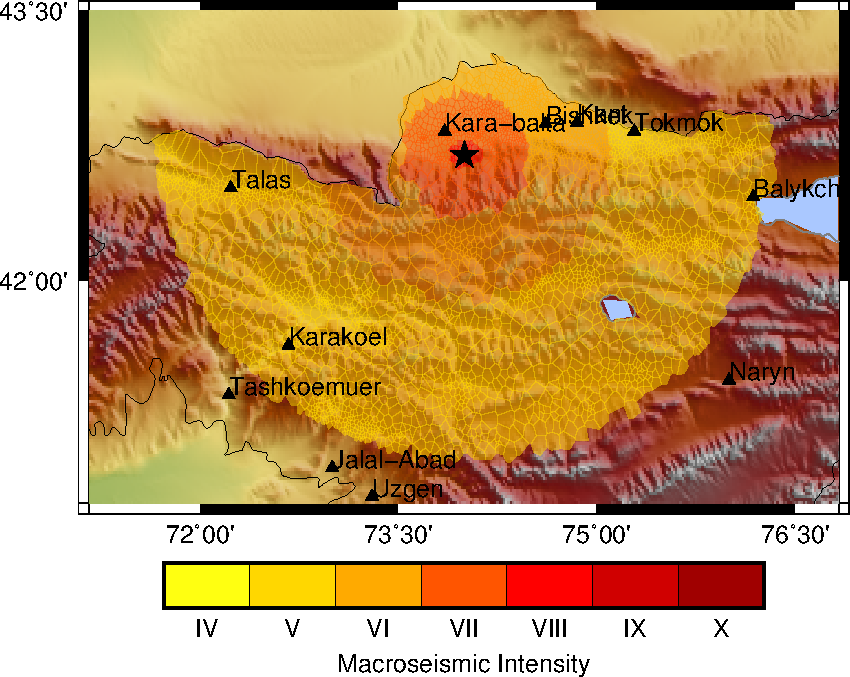
\includegraphics[width=12cm]{gm.pdf}
\caption{Estimated median macroseismic intensity}
\label{gm_fig}
\end{figure}


The maximum intensity, observed in geocell\_id \VAR{max_gm_loc} (usually in correspondence of the epicentre), is \VAR{max_gm}. The area where the earthquake could have been felt is approximately \VAR{area} qkm .
The maximum macroseismic intensity distribution for the largest affected settlement geocell\_id \VAR{largest} can be seen in Fig.\ref{gm_barplot}. 
Table\ref{fat_table} lists the median intensity expected in the \VAR{n} largest affected settlements.


\begin{figure}[h!]
\centering
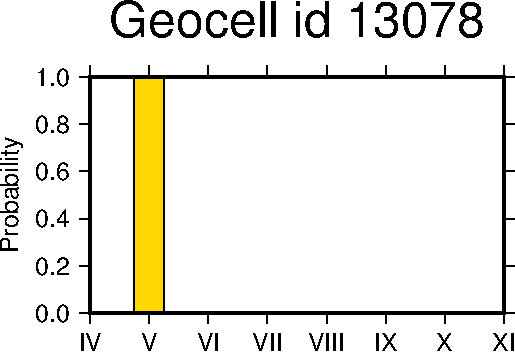
\includegraphics[width=8cm]{gm_barplot.pdf}
\caption{Estimated macroseismic intensity distribution}
\label{gm_barplot}
\end{figure}


\section*{Exposure}
The affected region can be characterized as an urban region.
Table\ref{bt_table} shows the \VAR{m} dominant residential building types in the target area and their relative percentage alongside their most likely vulnerability class.
The population has been disaggregated based on the relative frequencies and expected occupation of the residential buildings, in order to compute the estimated number of buildings.

\begin{table}[h!]
\caption{Building type distribution}
\label{bt_table}
\begin{tabular}{c|c|c}
\hline
EMCA{-}GEM Building Type&Relative&Most likely vulnerability\\
\hline
\BLOCK{for a,b,c in exposure}
\VAR{a} & \VAR{b} & \VAR{c} \\
\BLOCK{endfor}
\hline
\end{tabular}
\end{table}


\section*{Vulnerability and expected fatalities}
As we see from Table\ref{bt_table} the buildings within the region are mainly of vulnerability class\VAR{vc_string}.
Figure\ref{fat_fig} shows the expected distribution of casualties as forecasted by the CARAVAN system.
The sum of the median expected fatalities over the whole area is \VAR{fat_tot}.
Table\ref{fat_table} shows the most likely order of magnitude of fatalities in the \VAR{n} largest settlements in the affected area, the estimated population, and the estimated macroseismic intensity.


\begin{figure}[h!]
\centering
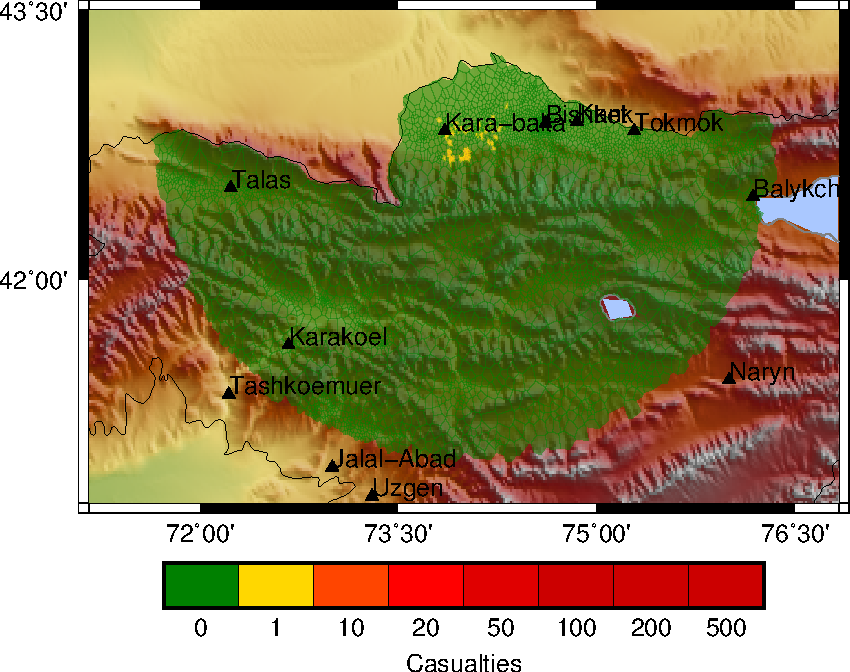
\includegraphics[width=12cm]{social.pdf}
\caption{Estimated loss distribution}
\label{fat_fig}
\end{figure}


\begin{table}[h!]
\caption{Table showing loss, estimated population and estmaied intensity for the 10 most affected locations}
\label{fat_table}
\begin{tabular}{c|c|c|c}
\hline
Geocell id&Expected casualties&Estimated population&Estimated intensity\\
\hline
\BLOCK{for a,b,c,d in loss}
\VAR{a} & \VAR{b} & \VAR{c} & \VAR{d} \\
\BLOCK{ endfor }
\hline
\end{tabular}
\end{table}


\section*{Disclaimer}
REWORD !!COPY PASTE FROM PAGER!! CARAVAN results are usually available shortly after an event. 
However, information on the extent of shaking will be uncertain in the minutes and hours following and earthquake and typically improves as additional data are available.
CARAVAN is regularly updated and users of CARAVAN hazard and loss estimates should account for uncertainty and always seek the most current CARAVAN release for any earthquake.
There will be infrequent cases where the CARAVAN estimates will be inaccurate, and even outside the stated range of the postulated uncertainties.
Population exposure is uncertain and varies by time of day, but these variations are not globally available so they are not currently considered for loss estimates in CARAVAN.
In addition, CARAVAN model loss calculations are approximate and may be inaccurate for some regions.
The uncertainties estimated for a given earthquake and for a particular CARAVAN version do not necessarily account for all the uncertainty associated with the estimated losses.
Potential errors or additional uncertainties in magnitude, location, depth, and shaking characteristics maybe not modeled explicitly and may remain unaccounted for in the CARAVAN loss{-}estimate ranges.
CARAVAN loss estimates also do not include losses due to tsunami or other secondary hazards (such as fire, liquefaction, and landsliding).
The CARAVAN system also does not completely account for aftershocks that may add to damage and losses.
Users of CARAVAN products should understand the potential uncertainties and or inaccuracies associated with CARAVAN's rapid loss{-}estimation capability: Individual or institutional users should use their own judgment and seek additional sources of information or advice before any decision making.


\end{document}
